%=============== PREAMBULO
% definicion de la clase del documento
\documentclass [oneside,10pt,titlepage]{beamer}

\mode<presentation>
{ % ==== Tema o fondo
  %\usetheme{Warsaw}
  %\usetheme{AnnArbor}
  %\usetheme{Antibes}
  %\usetheme{Bergen}
  %\usetheme{Berkeley}
  \usetheme{Berlin}
  %\usetheme{Boadilla}
  %\usetheme{CambridgeUS}
  %\usetheme{Copenhagen}
  %\usetheme{Darmstadt}
  %\usetheme{Dresden}
  %\usetheme{Frankfurt}
  %\usetheme{Goettingen}
  %\usetheme{Hannover}
  %\usetheme{Ilmenau}
  %\usetheme{JuanLesPins}
  %\usetheme{Luebeck}
  %\usetheme{Madrid}
  %\usetheme{Malmoe}
  %\usetheme{Marburg}
  %\usetheme{Montpellier}
  %\usetheme{PaloAlto}
  %\usetheme{Rochester}
  %\usetheme{Singapore}
  %\usetheme{Szeged}
% ==== Color de diapositiva
\usecolortheme[rgb={.10,.60,.30}]{structure}
% rojo verde azul
% rojo osc .9,.03,.01
%\usecolortheme{crane}
%\usecolortheme{albatross}
%\usecolortheme{beetle}
%\usecolortheme{dolphin}
%\usecolortheme{dove}
%\usecolortheme{fly}
%\usecolortheme{lily}
%\usecolortheme{orchid}
%\usecolortheme{rose}
%\usecolortheme{seagull}
%\usecolortheme{whale}
%\usecolortheme{seagull}
  \setbeamercovered{transparent}   % Para mostrar textos semitransparentes
}


% ============= Definicion de ambientes
\newtheorem{teorema}[theorem]{Teorema}


% ============= Paquetes
\usepackage[catalan]{babel}
\usepackage[latin1]{inputenc}
\usepackage{amssymb,amsfonts,amsbsy,latexsym}
%\usepackage[reqno]{amsmath}
\usepackage{graphicx}
\usepackage{epsfig}
\usepackage{dsfont}
\usepackage{textcomp}
\usepackage{ragged2e} % Paquete para justificar en los frame utilizando el comando /justifying
%\usepackage{times} % Paquete de tipo de letra, por defecto usa Computer Modern


% ============= Datos del documento
\title[PROBLEMAS 4 y 5]{PROBLEMAS 4 Y 5}


\subtitle{}
\author[Equipo 3]{Equipo 3}
\institute[]{Facultad de Matem\'aticas}
\date[dato corto]{4 de Noviembre de 2014}
\subject{Tema de la presentacion}



% =============== CUERPO DEL DOCUMENTO
\begin{document}


% =============== Crea titulo de la platica
\begin{frame}
  \titlepage
\end{frame}


% =============== Crea tabla de contenidos en funcion de las secciones y subsecciones
%\begin{frame}
%  \frametitle{Tabla de Contenido}
%  \tableofcontents[pausesections]  % TDC
%   You might wish to add the option [pausesections]
%\end{frame}


\justifying % Justifica el texto de los frame utilizando el paquete ragged2e

% =============== Aqui empieza la presentacion
\section{Problema 4}
\begin{frame}[allowframebreaks]

\begin{center}\textbf{Problema 4}\end{center}
\begin{block}{inciso a)}
Usando la definici�n de estabilidad determinar si la soluci�n del siguiente sistema es estable
\[
	3(t-1)\dot{x} = x, \qquad x(2)=0
\]
\end{block}

\begin{block}{Estabilidad de la soluci�n}
Primero que nada observamos que este sistema no es aut�nomo ya que depende expl�citamente de $t$, luego entonces no podemos aplicar la consabida teor�a de estabilidad.
\end{block}

\end{frame}

\begin{frame}[allowframebreaks]

\begin{block}{Soluci\'on}
Resolviendo por variables separables

\[
	\begin{array}{rcl}
		3(t-1)\frac{dx}{dt} & = & x\\
		\frac{1}{x} dx & = & \frac{1}{3}\frac{dt}{t-1}\\
		\ln x & = & \frac{1}{3}\ln(t-1) + c_1\\
		x & = & e^{\frac{1}{3}\ln(t-1) + c_1}\\
		& = & c_2 e^{\frac{1}{3}\ln(t-1)}\\
		& = & c_2 \sqrt[3]{t-1}
	\end{array}
\]
\end{block}
\end{frame}

\begin{frame}
\begin{block}{}
Aplicando la condici�n inicial $x(2)=0$

\[
	\begin{array}{c}
		x(2) = c_2 \sqrt[3]{2-1} = c_2 \cdot 1 = 0\\
		\Downarrow\\
		c_2 = 0
	\end{array}
\]

Quedando la soluci�n como $x(t) = 0$
\end{block}
\end{frame}

\begin{frame}
\begin{block}{inciso b)}
Usando la definici�n de estabilidad determinar si la soluci�n del siguiente sistema es estable
\[
	\begin{array}{c}
		\dot{x} = -x\\
		\dot{y} = -2y\\
		x(0) = y(0) = 0
	\end{array}
\]
\end{block}
\begin{block}{Soluci\'on}
Pasando el sistema de ecuaciones a una forma matricial tenemos:

\[
	\left(\begin{matrix}
		x\\
		y
	\end{matrix}\right)' =
	\left(\begin{matrix}
		-1 & 0 \\
		0 & -2
	\end{matrix}\right)
	\left(\begin{matrix}
		x \\
		y
	\end{matrix}\right)
\]

Dado que es una matriz diagonal $2 \times 2$ podemos saber r�pidamente que sus valores propios son

\[
	\begin{array}{rcl}
		\lambda_1 & = & -1 \\
		\lambda_2 & = & -2
	\end{array}
\]
\end{block}
\end{frame}

\begin{frame}
\begin{block}{}
Obteniendo sus vectores propios asociados, para $\lambda_1$ tenemos

\[
	\begin{array}{c}
		\left(\begin{matrix}
			0 & 0 \\
			0 & -1
		\end{matrix}\right)
		\left(\begin{matrix}
			a \\
			b
		\end{matrix}\right) = \left(\begin{matrix}
			0 \\
			0
		\end{matrix}\right) \\
		\downarrow \\
		b = 0 \\
		\downarrow \\
		v_1 = \left(\begin{matrix}
			1 \\
			0
		\end{matrix}\right)
	\end{array}
\]

Ahora para $\lambda_2$ se tiene

\[
	\begin{array}{c}
		\left(\begin{matrix}
			1 & 0 \\
			0 & 0
		\end{matrix}\right)\left(\begin{matrix}
			a \\
			b
		\end{matrix}\right) = \left(\begin{matrix}
			0 \\
			0
		\end{matrix}\right) \\
		\downarrow \\
		a = 0 \\
		\downarrow \\
		v_2 = \left(\begin{matrix}
			0 \\
			1
		\end{matrix}\right)
	\end{array}
\]
\end{block}
\end{frame}

\begin{frame}
\begin{block}{}
Finalmente la soluci�n del sistema quedar�a como

\[
	\left(\begin{matrix}
		x \\
		y
	\end{matrix}\right) = c_1 e^{-t}\left(\begin{matrix}
		1 \\
		0
	\end{matrix}\right) + c_2 e^{-2t}\left(\begin{matrix}
		0 \\
		1
	\end{matrix}\right)
\]

luego considerando la condici�n inicial

\[
	\begin{array}{c}
		\begin{array}{rcl}
			\left(\begin{matrix}
				x \\
				y
			\end{matrix}\right)(0) & = & c_1 e^0 \left(\begin{matrix}
				1 \\
				0
			\end{matrix}\right) + c_2 e^0 \left(\begin{matrix}
				0 \\
				1
			\end{matrix}\right) \\
			& = & c_1 \left(\begin{matrix}
				1 \\
				0
			\end{matrix}\right) + c_2 \left(\begin{matrix}
				0 \\
				1
			\end{matrix}\right)
		\end{array} \\
		\downarrow \\
		c_1 = c_2 = 0
	\end{array}
\]

Si observamos las ecuaciones originales podemos determinar el punto de equilibrio
\[
	\left(\begin{matrix}
		x \\
		y
	\end{matrix}\right)' = 0 \quad\Leftrightarrow\quad \left(\begin{matrix}
		x \\
		y
	\end{matrix}\right) = 0
\]
\end{block}
\end{frame}

\begin{frame}
\begin{block}{\textbf{Estabilidad de la soluci\'on}}

Es digno de observarse que si obtenemos el jacobiano de nuestro sistema de ecuaciones obtenemos la matriz original, debido a que el sistema ya es lineal.
\[
	J = \left(\begin{matrix}
		\frac{\partial (-x)}{\partial x} & \frac{\partial (-x)}{\partial y} \\
		\frac{\partial (-2y)}{\partial x} & \frac{\partial (-2y)}{\partial y}
	\end{matrix}\right) = \left(\begin{matrix}
		-1 & 0 \\
		0 & -2
	\end{matrix}\right)
\]

Finalmente observando los valores propios de la matrix $\lambda_1 = -1$, $\lambda_2 = -2$ podemos decir que puesto que ambos son negativos el �nico punto de equilibrio debe ser estable.

\end{block}
\end{frame}

\section{Problema 5}

\begin{frame}
\begin{block}{Problema 5}
Convertir en un sistema de ecuaciones y realizar el estudio completo del sistema restante:
\begin{equation}
x'' + k \sin x = 0 \hspace{20pt} k>0
\end{equation}
\end{block}
\end{frame}

\begin{frame}
\begin{block}{Soluci\'on}
Tomemos el siguiente cambio de variable:
\begin{equation}
\begin{split}
y_{1}=x & \Rightarrow y_{1}'=x'=y_{2} \\
y_{2}=x' & \Rightarrow y_{2}'=x''= -k\sin x 
\end{split}
\end{equation}
As\'i, resulta el siguiente sistema de ecuaciones diferenciales:
\begin{equation}
\begin{split}
y_{1}' & = y_{2}\\
y_{2}' & = -k\sin y_{1}
\end{split}
\end{equation}
\end{block}
\end{frame}

\begin{frame}
Observemos las siguientes propiedades:
\begin{itemize}
\item El sistema (3) es aut\'onomo, ya que NO depende expl\'icitamente de $t$
\item El sistema (3) es no-lineal, ya que en la segunda ecuaci\'on del sistema hay una funci\'on seno que depende de la variable $x$
\end{itemize}
\end{frame}

\begin{frame}
Ceroclinas del sistema (3):
\begin{equation}
\begin{split}
y_{2} = 0\\
-k\sin y_{1} = 0
\end{split}
\end{equation}
Es decir, el conjunto de puntos de equilibrio de (3) es el siguiente:
\begin{equation}
\{((2n) \pi, 0) | n \in \mathbb{Z}\}
\end{equation}
\end{frame}

\begin{frame}
\begin{center} \textbf{An\'alisis de estabilidad} \end{center}
La matriz Jacobiana del sistema queda de la siguiente forma:
\[
J(y_{1},y_{2})=
\begin{pmatrix}
0 & 1\\
-k \cos y_{1} & 0
\end{pmatrix}
\]
Evaluando los puntos de equilibrio en J:
\[
J((2n) \pi,0)=
\begin{pmatrix}
0 & 1\\
-k & 0
\end{pmatrix}
\]

\begin{equation}
P(\lambda) = \lambda ^{2} + k
\end{equation}
El polinomio caracter\'istico nos dice que tenemos dos valores propios imaginarios $\pm ki$ (parte real cero), es decir, tenemos centros como se muestra en la figura \ref{fig:orbitas}

\end{frame}

\begin{frame}

\begin{figure}
	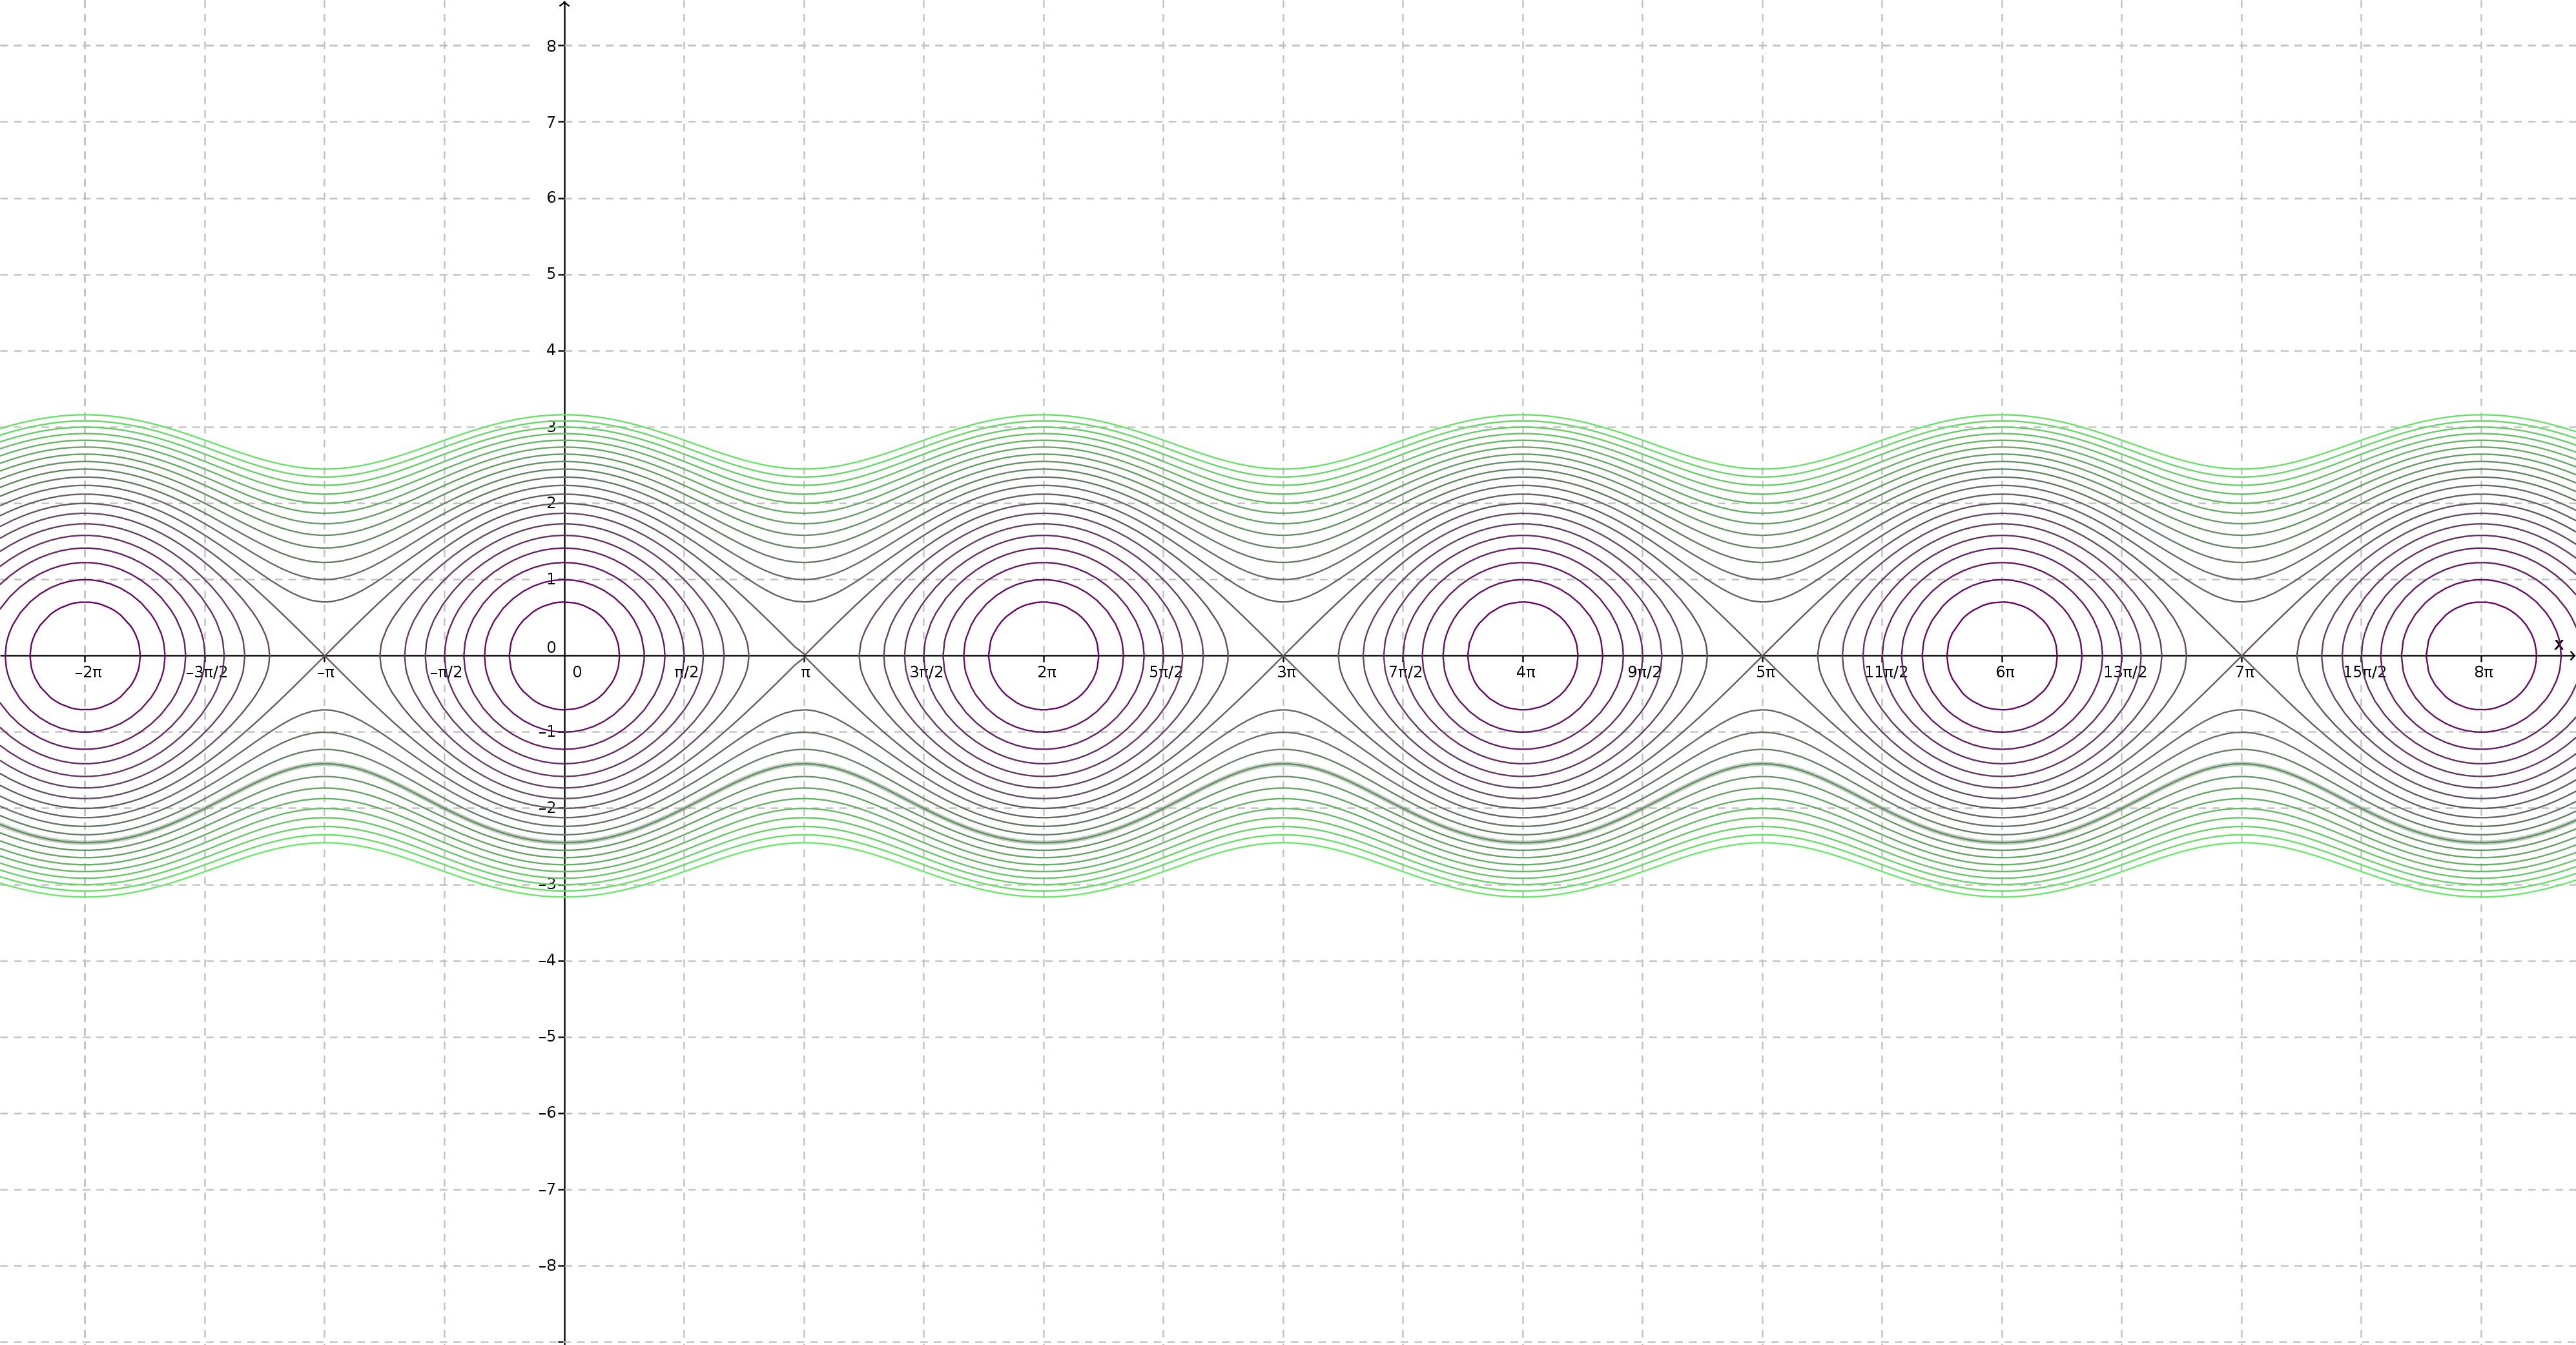
\includegraphics[width=\textwidth]{plot.png}
	\caption{�rbitas alrededor de los puntos de equilibrio con $k=1$}
	\label{fig:orbitas}
\end{figure}

\end{frame}

\begin{frame}

N�tese que si var�a el par�metro $k$ de la ecuaci�n tenemos gr�ficas m�s alargadas

\begin{figure}
	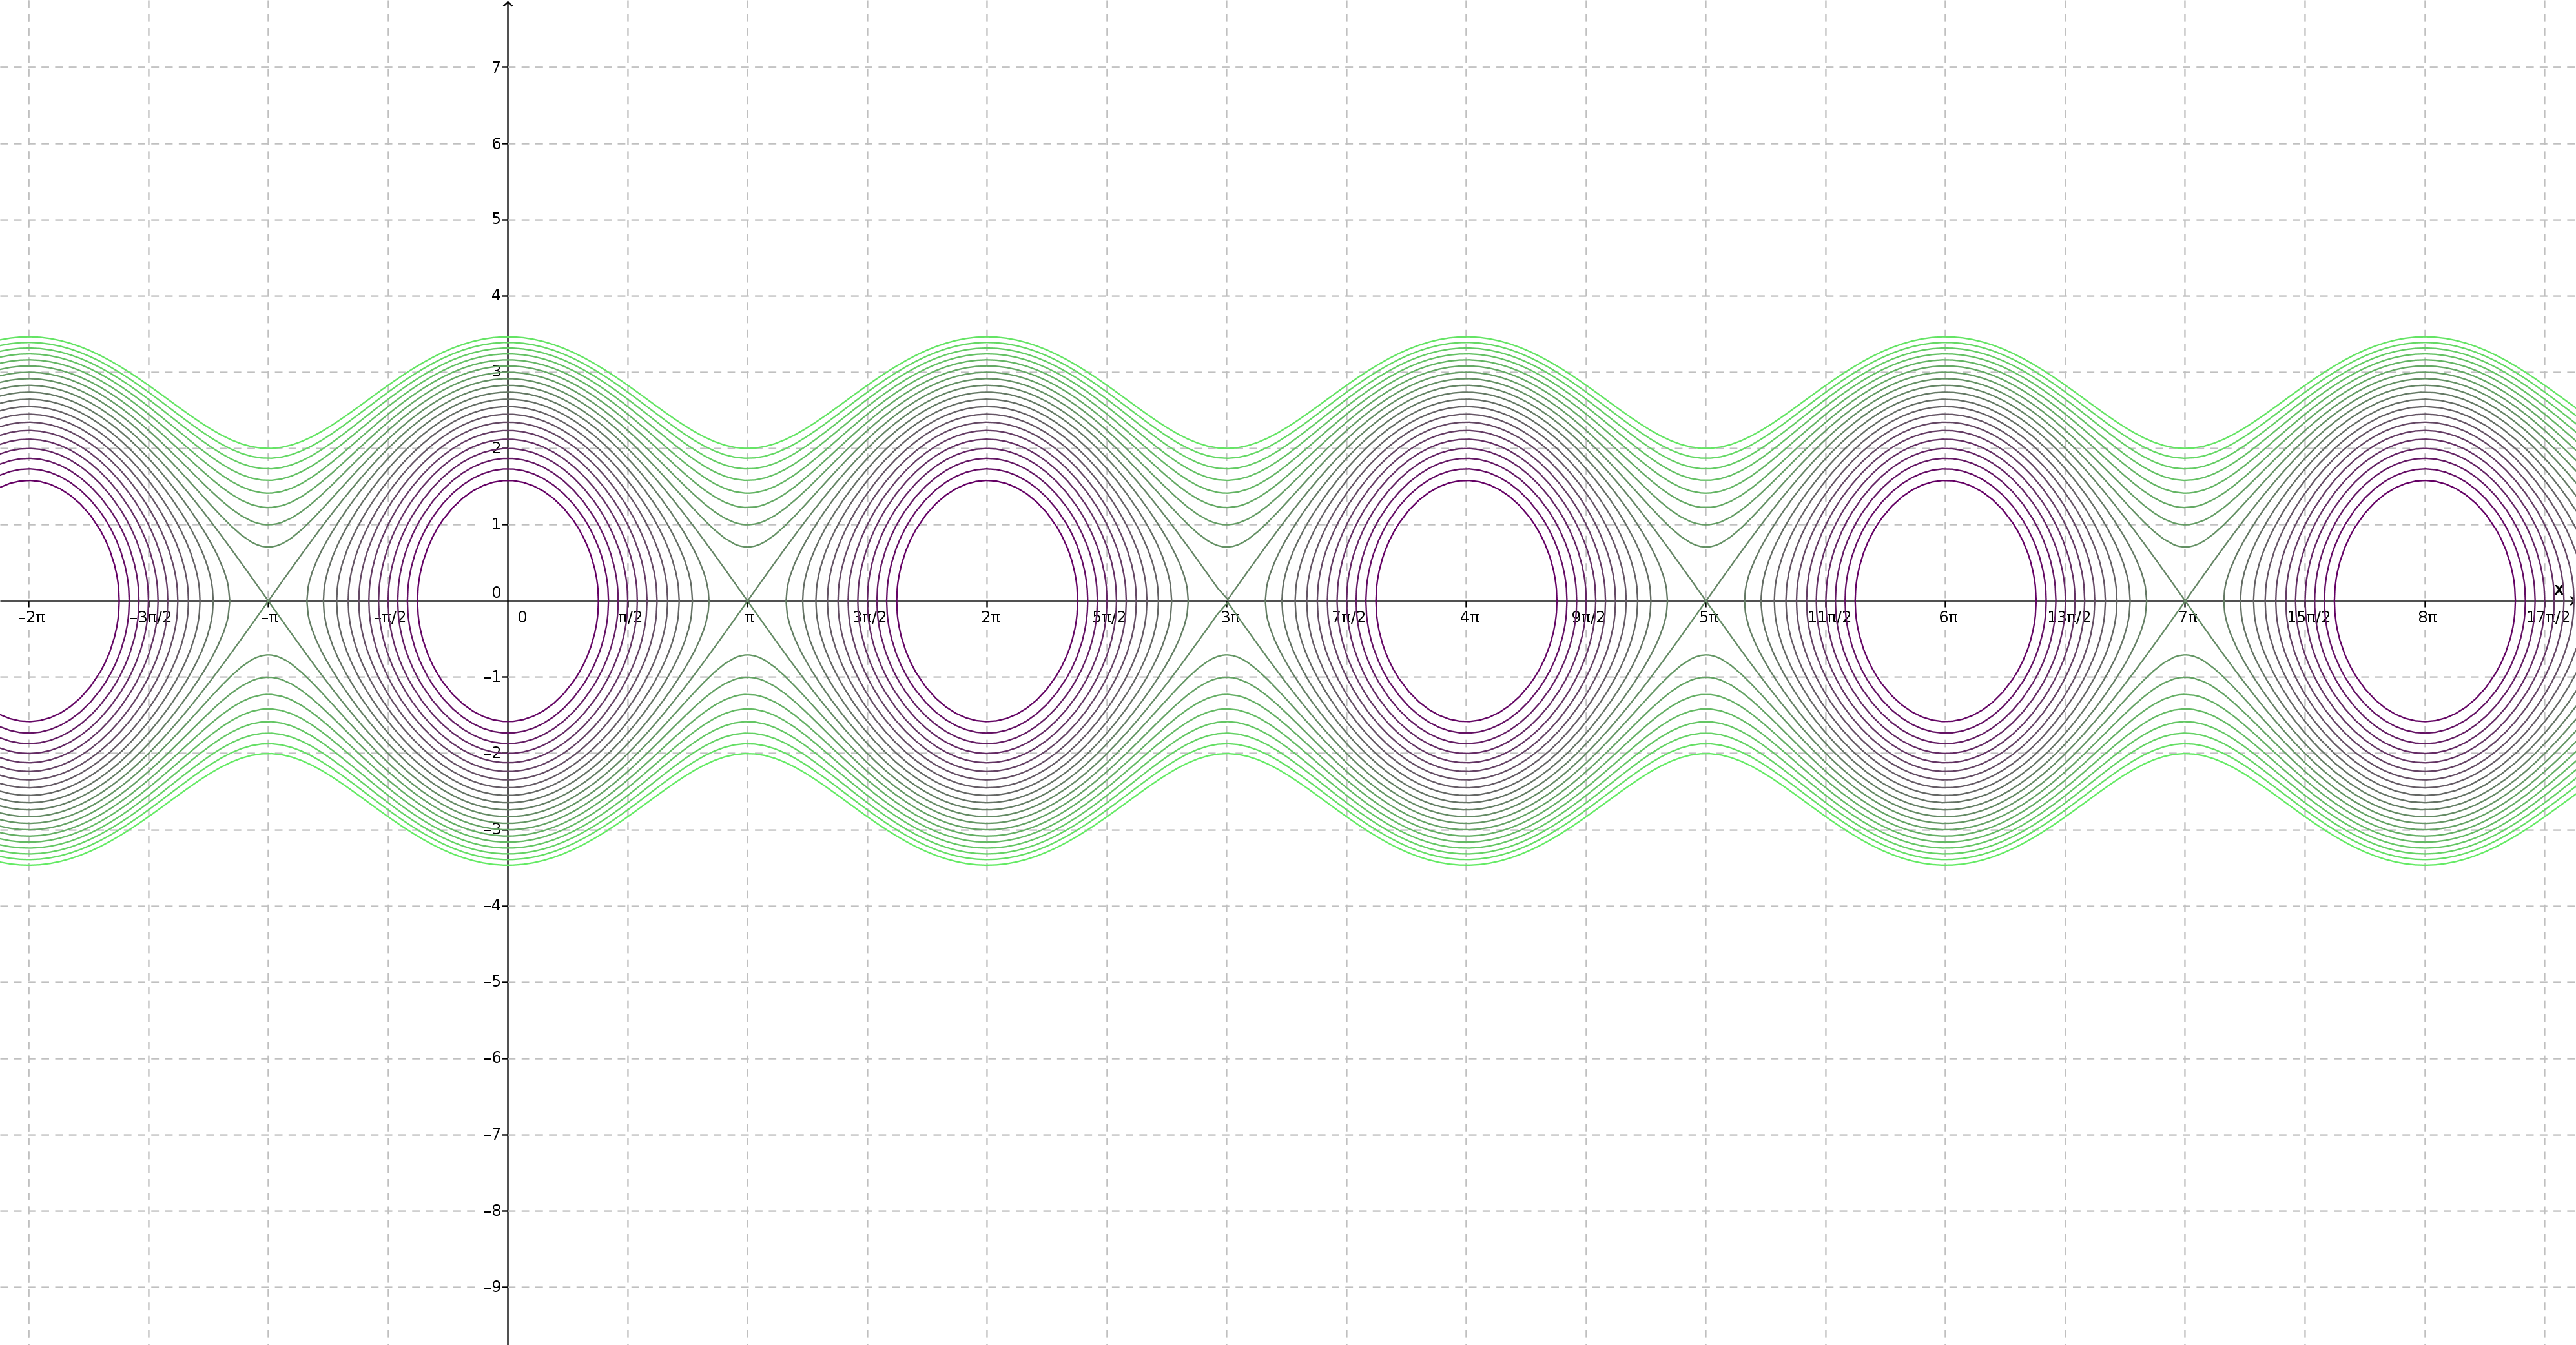
\includegraphics[width=\textwidth]{plot2.png}
	\caption{Variando $k=2$}
	\label{fig:orbitas_largas}
\end{figure}

\end{frame}

\end{document}